\chapter{Diseño e implementación}
Una vez diseñada la arquitectura de la plataforma, es necesario detallar el proceso de creación de cada una de las unidades de las que consta la aplicación. Para ello, en primer lugar, se explicará como está organizado y desarrollado el módulo de Python de los test estadísticos. En segundo lugar, se detallará el diseño de la API REST desde el punto de vista de las URIs que conforman cada servicio web. Por último, se detallará la capa superior de la arquitectura, explicando cómo será la interfaz gráfica mediante prototipado y analizando su nivel de usabilidad mediante los principios heurísticos de Nielsen. Así mismo, se hará uso de UML para especificar los diagramas de secuencia de las funcionalidades más relevantes del sistema.

\section{Módulo Python test estadísticos} \label{dis_py}
El módulo de Python de los test estadísticos o módulo STAC (Statistical Tests for Algorithm Comparison) está formado por los siguientes archivos:
\begin{itemize}
\item \textbf{tests\_parametricos.py:} contiene el test paramétrico ANOVA y el test POST-HOC de Bonferroni para el test de ANOVA.
\item \textbf{tests\_no\_parametricos.py:} contiene todos los test no paramétricos (Wilcoxon, Friedman, etc.) indicados en los objetivos del proyecto, excepto aquellos que ya se encuentran en la librería SciPy, tal y como se indicó en la sección \ref{libreriastest}.
\item \textbf{\_\_init\_\_.py:} para que los archivos de test puedan ser importados todos a la vez, es posible empaquetarlos juntos. En este fichero se indica qué se importará al importar el módulo.
\end{itemize}
Este módulo, como se había comentado en la sección \ref{nonparametric} del capítulo \ref{arquitecturayh}, tiene dependencias con la librería SciPy (con el módulo \textit{stats}), así como con el paquete NumPy. La funcionalidad de SciPy sirve a este proyecto para poder hallar parámetros básicos que serán necesarios para obtener todos los datos necesarios en los test.

El diseño del los test estadísticos está determinado por los argumentos de entrada y valores de salida cada test.

\subsection{Test paramétricos}

\noindent
\textbf{Prototipo de la función del test ANOVA:}

\texttt{anova\_test(matriz\_datos, alpha=0.05)}

\begin{itemize}
\item \textbf{``matriz\_datos":} lista de listas de conjuntos de datos. Cada conjunto de datos representa los resultados obtenidos por los algoritmos al ser aplicados sobre un problema concreto.
\item \textbf{``alpha":} nivel de significación o error tipo I (probabilidad de rechazar la hipótesis nula siendo cierta).
\end{itemize}

\noindent
\textbf{Datos devueltos:}

Diccionario que contiene los siguientes datos:

\begin{itemize}
\item \textbf{``resultado":} \textit{true} ó \textit{false}, que indica que el contraste es estadísticamente significativo o estadísticamente no significativo, dependiendo de si el p\_valor es menor que el nivel de significación.
\item \textbf{``p\_valor":} probabilidad de obtener un valor al menos tan extremo como el estadístico hallado suponiendo la hipótesis nula cierta.
\item \textbf{``estadístico":} valor del estadístico en cuestión.
\item \textbf{``variaciones":} lista con las variaciones o sumas de cuadrados total, entre tratamientos y variación del error (SCT, SCTR, SCE).
\item \textbf{``grados\_libertad":} lista con los grados de libertad totales, entre tratamientos y del error (GLT, GLTR, GLE).
\item \textbf{``cuadrados\_medios":} lista con los cuadrados medios (suma cuadrados / grados libertad) total, entre tratamientos y variación del error (SCT, SCTR, SCE).
\item \textbf{``medias\_algoritmos":} lista con las medias de los datos de cada tratamiento o algoritmo.
\item \textbf{``media\_general":} media de la lista de medias de los algoritmos.
\end{itemize}

\noindent
\textbf{Prototipo de la función del test POST-HOC Bonferroni:}

\texttt{bonferroni\_test(nombres\_algoritmos, medias\_algoritmos, cuadrado\_medio\_error, N, alpha=0.05)}

\begin{itemize}
\item \textbf{``nombres\_algoritmos":} lista de los nombres de los algoritmos.
\item \textbf{``medias\_algoritmos":} lista con las medias de los datos de cada tratamiento o algoritmo.
\item \textbf{``cuadrado\_medio\_error":} valor del cuadrado medio del error (suma cuadrados error / grados libertad error).
\item \textbf{``N":} número de conjuntos de datos.
\item \textbf{``alpha":} nivel de significación o error tipo I (probabilidad de rechazar la hipótesis nula siendo cierta).
\end{itemize}

\noindent
\textbf{Datos devueltos:}

Diccionario que contiene los siguientes datos:

\begin{itemize}
\item \textbf{``resultado":} lista de valores \textit{true} ó \textit{false}, que indica si cada uno de los contrastes es o no estadísticamente significativo, dependiendo de si cada uno de los p\_valores es menor que el nivel de significación.
\item \textbf{``p\_valores":} lista de probabilidades de obtener un valor al menos tan extremo como cada uno de los estadísticos hallados suponiendo la hipótesis nula cierta.
\item \textbf{``valores\_t":} lista de valores o estadísticos para cada comparación.
\item \textbf{``p\_valores ajustados":} lista de los p\_valores de las comparaciones ajustados a toda la familia de comparaciones.
\item \textbf{``alpha":} nivel de significación (modificado según el valor de m).
\item \textbf{``comparaciones":} lista donde cada elemento es un texto que contiene los nombres de los dos algoritmos involucrados en la comparación tal como “algoritmoA vs algoritmoB”. Se ordena según del p\_valor de la comparación.
\end{itemize}

\subsection{Test no paramétricos}

\noindent
\textbf{Prototipos de la función del test no paramétricos de Wilcoxon:}

\texttt{wilcoxon\_test(matriz\_datos, alpha=0.05)}

\begin{itemize}
\item \textbf{``matriz\_datos":} lista de listas de conjuntos de datos. Cada conjunto de datos representa los resultados obtenidos por los algoritmos al ser aplicados sobre un problema concreto.
\item \textbf{``alpha":} nivel de significación o error tipo I (probabilidad de rechazar la hipótesis nula siendo cierta).
\end{itemize}

\noindent
\textbf{Datos devueltos:}

Diccionario que contiene los siguientes datos:

\begin{itemize}
\item \textbf{``resultado":} \textit{true} ó \textit{false}, que indica que el contraste es estadísticamente significativo o estadísticamente no significativo, dependiendo de si el p\_valor es menor que el nivel de significación.
\item \textbf{``estadistico":} valor del estadístico en cuestión.
\item \textbf{``suma rangos pos":} suma de los rangos de las diferencias mayores que 0.
\item \textbf{``suma rangos neg":} suma de los rangos de las diferencias menores que 0.
\item \textbf{Si $N \leq 25$ (tamaño muestral):}
\subitem \textbf{- ``punto critico"} límite inferior del intervalo de aceptación. El contraste será estadísticamente significativo si: estadístico $\leq$ límite inferior correspondiente.
\item \textbf{Si $N > 25$:}
\subitem \textbf{- ``p\_valor":} probabilidad de obtener un valor al menos tan extremo como el estadístico hallado suponiendo la hipótesis nula cierta.
\end{itemize}

\noindent
\textbf{Prototipos de las funciones test no paramétricos de ranking:}

\texttt{friedman\_test(nombres\_algoritmos, matriz\_datos, alpha=0.05, tipo=0)}

\texttt{iman\_davenport\_test(nombres\_algoritmos, matriz\_datos, alpha=0.05, tipo=0)}

\texttt{friedman\_rangos\_alineados\_test(nombres\_algoritmos, matriz\_datos, alpha=0.05, tipo=0)}

\texttt{quade\_test(nombres\_algoritmos, matriz\_datos, alpha=0.05, tipo=0)}

\begin{itemize}
\item \textbf{``nombres\_algoritmos":} lista que contiene los nombres de los algoritmos y que será empleada para devolver el ranking de nombres de los algoritmos.
\item \textbf{``matriz\_datos":} lista de listas de conjuntos de datos. Cada conjunto de datos representa los resultados obtenidos por los algoritmos al ser aplicados sobre un problema concreto.
\item \textbf{``alpha":} nivel de significación o error tipo I (probabilidad de rechazar la hipótesis nula siendo cierta).
\item \textbf{``tipo":} indica si lo que se pretende es minimizar (en cuyo caso se establece a 0) o maximizar (se establece a 1).
\end{itemize}

\noindent
\textbf{Datos devueltos:}

Diccionario que contiene los siguientes datos:

\begin{itemize}
\item \textbf{``resultado":} \textit{true} ó \textit{false}, que indica que el contraste es estadísticamente significativo o estadísticamente no significativo, dependiendo de si el p\_valor es menor que el nivel de significación.
\item \textbf{``p\_valor":} probabilidad de obtener un valor al menos tan extremo como el estadístico hallado suponiendo la hipótesis nula cierta.
\item \textbf{``estadistico":} valor del estadístico en cuestión.
\item \textbf{``nombres":} lista de los nombres de los algoritmos ordenados según los valores numéricos de los rankings medios obtenidos por los distintos algoritmos.
\item \textbf{``ranking":} lista de los valores de los rankings medios ordenados de menor a mayor (cuanto menor es el valor mejor es el dato.)
\end{itemize}

\noindent
\textbf{Prototipos de las funciones de los test POST-HOC:}

\texttt{bonferroni\_dunn\_test(K, nombres, valores\_z, p\_valores, metodo\_control, alpha=0.05)}

\texttt{holm\_test(K, nombres, valores\_z, p\_valores, metodo\_control, alpha=0.05)}

\texttt{hochberg\_test(K, nombres, valores\_z, p\_valores, metodo\_control, alpha=0.05)}

\texttt{li\_test(K, nombres, valores\_z, p\_valores, metodo\_control, alpha=0.05)}

\texttt{finner\_test(K, nombres, valores\_z, p\_valores, metodo\_control, alpha=0.05)}

\texttt{nemenyi\_multitest(m, comparaciones, valores\_z, p\_valores, alpha=0.05)}

\texttt{holm\_multitest(m, comparaciones, valores\_z, p\_valores, alpha=0.05)}

\texttt{hochberg\_multitest(m, comparaciones, valores\_z, p\_valores, alpha=0.05)}

\texttt{finner\_multitest(m, comparaciones, valores\_z, p\_valores, alpha=0.05)}

\texttt{shaffer\_multitest(m, comparaciones, valores\_z, p\_valores, alpha=0.05)}

\begin{itemize}
\item \textbf{``K":} número de algoritmos (incluyendo método de control).
\item \textbf{``valores\_z":} estadísticos calculados en función del test de ranking y del ranking devuelto por el test principal. Siguen una normal (0, 1) y están ordenados según los p\_valores.
\item \textbf{``p\_valores":} p-valores de cada uno de los estadísticos para comparar con los niveles de significancia ajustados.
\item \textbf{``nombres":} lista de nombres de los algoritmos (con los que el método de control se compara) ordenados según los p\_valores.
\item \textbf{``metodo\_control":} método de control del test, por convención es el test de menor ranking.
\item \textbf{``alpha":} nivel de significancia (probabilidad de error tipo 1) del test de ranking principal.
\item \textbf{``m":} número de comparaciones.
\item \textbf{``comparaciones":} nombres de las hipótesis contrastadas. Por ejemplo “algoritmoA vs algoritmoB”.
\end{itemize}

\noindent
\textbf{Datos devueltos:}

Diccionario que contiene los siguientes datos:                                              

\begin{itemize}
\item \textbf{``valores\_z"} y \textbf{``p\_valores"}.
\item \textbf{``alpha" \space ó ``alphas":} nivel de significación. Bonferroni-Dunn y Li devuelven un alpha modificado. El resto de test devuelven una lista de alphas cuyos elementos son diferentes para cada comparación.
\item \textbf{``resultado":} lista de valores \textit{true} ó \textit{false}, que indica si cada uno de los contrastes es o no estadísticamente significativo, dependiendo de si cada uno de los p\_valores es menor que el nivel de significación.
\item \textbf{``p\_valores ajustados":} lista de los p\_valores de las comparaciones ajustados a toda la familia de comparaciones.
\end{itemize}

Para los test con método de control, el diccionario también incluye \textbf{``metodo\_control"} y \textbf{``nombres"}. Para los test de comparación múltiple, éste también incluye: \textbf{``comparaciones"}.

\section{API Servicios REST} \label{dis_api}
Como se había comentado en la sección \ref{bottle} del capítulo \ref{arquitecturayh}, Bottle permite la implementación de servicios web accesibles mediante una o más URIs (\textit{Uniform Resource Identifier} o identificador de recursos uniforme). El decorador \textit{route()} asigna una URI a un trozo de código (el propio servicio web) en lo que se denomina ruta. El diseño de la API REST está determinado por las URIs mediante las cuales se puede acceder a los servicios.

La plataforma cuenta con una API REST en la que se distinguen dos tipos de servicios web, diferenciados por la utilidad que tienen:
\begin{itemize}
\item Servicios de subida / consulta de ficheros de datos.
\item Servicios de acceso / ejecución de los test.
\end{itemize}

Para los ejemplos de URIs en el diseño se supone que todos los servicios escuchan en /api/. Esto se pudo hacer modificando el archivo que utiliza el módulo WSGI para cargar la aplicación (API REST) en el servidor web Apache. En el manual técnico del presente documento (manual de despliegue) se detallará el contenido de este archivo.

\textbf{Servicios de subida y consulta de ficheros:} Podemos ver el diseño de este tipo de servicios en los cuadros \ref{cuadro1} y \ref{cuadro2}. El primer decorador permite la subida y el almacenamiento del contenido de un fichero en el servidor. El método usado es ``POST", ya que se envían datos al servidor (el fichero) y éste devuelve el resumen HASH del contenido del fichero o error en el caso de que se haya producido algún error en el procesamiento del archivo o éste no se encuentre en el servidor. El segundo decorador, permite consultar los datos de un fichero en concreto. Tiene un parámetro de entrada no opcional \textit{id\_fichero} (resumen HASH del contenido del fichero). En caso de no existir un fichero con esa clave, se devuelve error. El método empleado es ``GET", ya que únicamente se reciben datos del servidor.

\begin{table}[H]
	\centering
	\begin{tabular}{|l|}
		\hline
		\multicolumn{1}{|c|}{\textbf{Decorador}} \\ \hline
		\texttt{@route('/fichero', method="POST")} \\ \hline
		\texttt{@route('/fichero/<id\_fichero>', method="GET")} \\ \hline
	\end{tabular}
	\caption{Decoradores Bottle.}
	\label{cuadro1}
\end{table}

\begin{table}[H]
	\centering
	\begin{tabular}{|l|c|}
		\hline
		\multicolumn{1}{|c|}{\textbf{Ejemplo URI}} & {\textbf{Método}} \\ \hline
		\texttt{http://localhost/api/fichero} & \texttt{POST} \\ \hline
		\texttt{http://localhost/api/fichero/id\_fichero} & \texttt{GET} \\ \hline
	\end{tabular}
	\caption{Ejemplos de URIs y métodos empleados.}
	\label{cuadro2}
\end{table}

\textbf{Servicios de acceso y ejecución de test:} Estos servicios son los encargados de dar acceso a la ejecución de los test estadísticos y los que devuelven los datos proporcionados por éstos (en formato JSON) al navegador. La función AJAX de jQuery se encargará de mostrar estos datos en la interfaz de usuario. El método empleado es GET, ya que los servicios web de los test únicamente devuelven datos (resultado de su ejecución).

Los cuadros \ref{cuadro3} y \ref{cuadro4} muestran el diseño para los test de evaluación de las condiciones paramétricas, los test paramétricos y el test de Wilcoxon (no paramétrico):

\begin{table}[H]
	\centering
	\begin{tabular}{|l|}
		\hline
		\multicolumn{1}{|c|}{\textbf{Decorador}} \\ \hline
		\texttt{@route('/nombre/<id\_fichero>', method="GET")} \\ \hline
		\texttt{@route('/nombre/<id\_fichero>/<alpha:float>', method="GET") } \\ \hline
	\end{tabular}
	\caption{Decoradores Bottle.}
	\label{cuadro3}
\end{table}

\begin{table}[H]
	\centering
	\begin{tabular}{|l|c|}
		\hline
		\multicolumn{1}{|c|}{\textbf{Ejemplo URI}} & {\textbf{Método}} \\ \hline
		\texttt{http://localhost/api/ttest/id\_fichero} & \texttt{GET} \\ \hline
		\texttt{http://localhost/api/ttest/id\_fichero/0.05} & \texttt{GET} \\ \hline
	\end{tabular}
	\caption{Ejemplos de URIs y métodos empleados.}
	\label{cuadro4}
\end{table}

El valor \textit{nombre} indica el nombre del test referenciado (p. ej. /ttest/...) Los parámetros utilizados son los siguientes:
\begin{itemize}
\item \textbf{alpha:} nivel de significación. Parámetro opcional cuyo valor por defecto es 0.05 (probabilidad de error tipo 1 más común).
\item \textbf{id\_fichero:} resumen HASH del contenido del fichero que identifica al mismo inequívocamente. Se trata de un parámetro no opcional.
\end{itemize}

Los cuadros \ref{cuadro5} y \ref{cuadro6} muestran el diseño para los test no paramétricos de ranking (como el test de Friedman, el test de Iman-Davenport, etc.):

\begin{table}[H]
	\centering
	\begin{tabular}{|l|}
		\hline
		\multicolumn{1}{|c|}{\textbf{Decorador}} \\ \hline
		{\small \texttt{@route('/nombre/<id\_fichero>/<test\_comparacion>', method="GET")}} \\ \hline
		{\small \texttt{@route('/nombre/<id\_fichero>/<alpha:float>/<test\_comparacion>', method="GET")}} \\ \hline
		{\small \texttt{@route('/nombre/<id\_fichero>/<tipo:int>/<test\_comparacion>', method="GET")}} \\ \hline
		{\small \texttt{@route('/nombre/<id\_fichero>/<alpha:float>/<tipo:int>/<test\_comparacion>', method="GET")}} \\ \hline
		{\small \texttt{@route('/nombre/<id\_fichero>', method="GET")}} \\ \hline
		{\small \texttt{@route('/nombre/<id\_fichero>/<alpha:float>', method="GET")}} \\ \hline
		{\small \texttt{@route('/nombre/<id\_fichero>/<tipo:int>', method="GET")}} \\ \hline
		{\small \texttt{@route('/nombre/<id\_fichero>/<alpha:float>/<tipo:int>', method="GET")}} \\ \hline
	\end{tabular}
	\caption{Decoradores Bottle.}
	\label{cuadro5}
\end{table}

\begin{table}[H]
	\centering
	\begin{tabular}{|l|c|}
		\hline
		\multicolumn{1}{|c|}{\textbf{Ejemplo URI}} & {\textbf{Método}} \\ \hline
		\texttt{http://localhost/api/friedman/id\_fichero/li\_test} & \texttt{GET} \\ \hline
		\texttt{http://localhost/api/friedman/id\_fichero/0.05/li\_test} & \texttt{GET} \\ \hline
		\texttt{http://localhost/api/friedman/id\_fichero/1/li\_test} & \texttt{GET} \\ \hline
		\texttt{http://localhost/api/friedman/id\_fichero/0.05/1/li\_test} & \texttt{GET} \\ \hline
		\texttt{http://localhost/api/friedman/id\_fichero} & \texttt{GET} \\ \hline
		\texttt{http://localhost/api/friedman/id\_fichero/0.05} & \texttt{GET} \\ \hline
		\texttt{http://localhost/api/friedman/id\_fichero/1} & \texttt{GET} \\ \hline
		\texttt{http://localhost/api/friedman/id\_fichero/0.05/1} & \texttt{GET} \\ \hline
	\end{tabular}
	\caption{Ejemplos de URIs y métodos empleados.}
	\label{cuadro6}
\end{table}

El valor \textit{nombre} indica el nombre del test de ranking referenciado (p. ej. /friedman/...) Los parámetros utilizados son los siguientes:
\begin{itemize}
\item \textbf{alpha:} nivel de significación. Parámetro opcional cuyo valor por defecto es 0.05 (probabilidad de error tipo 1 más común).
\item \textbf{tipo:} indica la función objetivo de los algoritmos a contrastar: minimización (0) / maximización (1). Es un parámetro opcional cuyo valor por defecto es 0 (minimización).
\item \textbf{test\_comparacion:} indica el nombre del test POST-HOC a aplicar en caso de que el resultado del test de ranking determine que existen diferencias significativas. Se trata de un parámetro opcional cuyo valor por defecto es ``bonferroni\_dunn\_test".
\item \textbf{id\_fichero:} resumen HASH del contenido del fichero que identifica al mismo inequívocamente. Se trata de un parámetro no opcional.
\end{itemize}

\section{Aplicación web}
\subsection{Prototipo de la interfaz gráfica}
Para la implementación de la interfaz gráfica se construyeron inicialmente varios prototipos visuales de diferentes aspectos de la plataforma para luego poder proceder a su implementación. Para elaborar estos prototipos, se tuvieron en cuenta las historias de usuario del cliente vistas en la sección \ref{hu_cliente} del capítulo \ref{analisisreq}. En las figuras \ref{fig:prot_home}, \ref{fig:prot_help}, \ref{fig:prot_test} y \ref{fig:prot_results} podemos ver los prototipos de la página principal, la página donde se muestra la ayuda, la página de selección de parámetros de los test y la página de visualización de los resultados respectivamente. Por otro lado, en el manual de usuario al final del presente documento se muestra en las figuras \ref{fig:man_inicio}, \ref{fig:man_ayuda2}, \ref{fig:man_opciones} y \ref{fig:man_results} el resultado final de la implementación.

\begin{figure}[H]
\centering
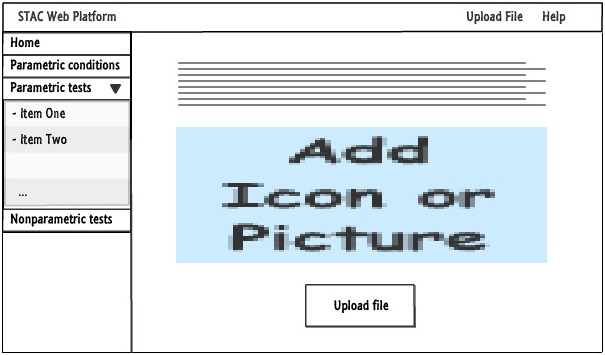
\includegraphics[width=10cm,height=6cm]{figuras/prototipo_home.jpg}
\caption{Prototipo de página principal.}
\label{fig:prot_home}
\end{figure}

\begin{figure}[H]
\centering
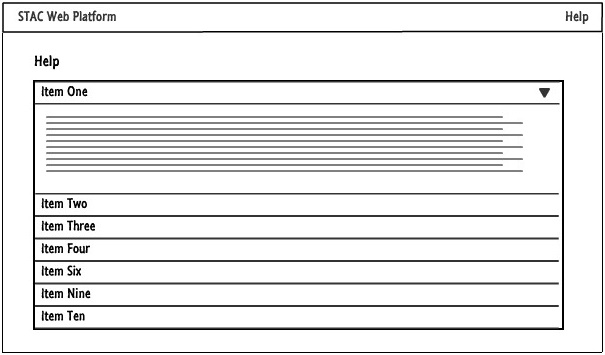
\includegraphics[width=10cm,height=6cm]{figuras/prototipo_help.jpg}
\caption{Prototipo página de ayuda.}
\label{fig:prot_help}
\end{figure}

\begin{figure}[H]
\centering
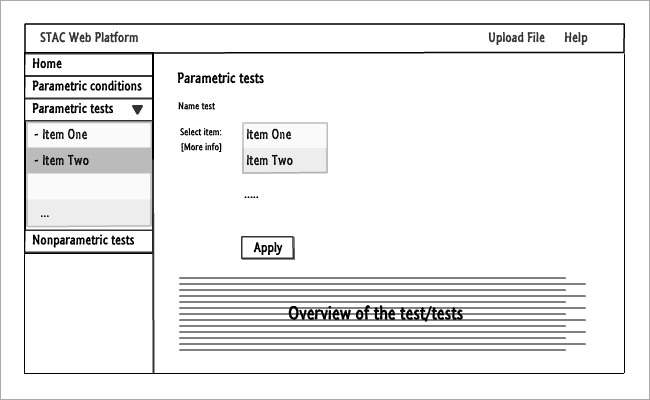
\includegraphics[width=10cm,height=6cm]{figuras/prototipo_test.jpg}
\caption{Prototipo página selección de parámetros/opciones.}
\label{fig:prot_test}
\end{figure}

\begin{figure}[H]
\centering
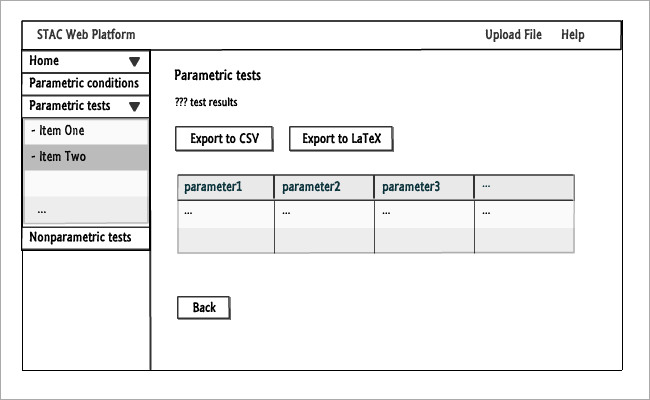
\includegraphics[width=10cm,height=6cm]{figuras/prototipo_results.jpg}
\caption{Prototipo página visualización de resultados.}
\label{fig:prot_results}
\end{figure}

\subsection{Heurísticas de Nielsen}
En la interacción persona-ordenador, se siguen varios pasos para crear sistemas que sean amigables para el usuario. En el paso de evaluación, se pueden realizar pruebas de expertos, en las cuales lo más común es utilizar las heurísticas creadas por Jakob Nielsen para evaluar el diseño de la interfaz de usuario. Los 10 principios de diseño basados en el usuario, que definió Jakob Nielsen en 1990, siguen siendo un referente importante para evaluar la usabilidad de un sitio web. A
continuación se detallan los principios heurísticos de Nielsen, y se comenta en qué medida el sistema cumple con estos principios.

\noindent
\textbf{Visibilidad del estado del sistema}

\textit{El sistema debe siempre mantener a los usuarios informados del estado del sistema, con una realimentación apropiada y en un tiempo razonable.}

El sistema siempre trata de indicar el lugar donde se encuentra el usuario, así como las acciones que puede realizar en el lugar en el que se encuentre. La parte superior de la web trata de indicar estos aspectos mediante títulos / breves descripciones. El menú desplegable de la izquierda también proporciona información del lugar en el que se encuentra el usuario.

\noindent
\textbf{Lenguaje de los usuarios}

\textit{El sistema debe hablar el lenguaje de los usuarios, con las palabras, las frases y los conceptos familiares, en lugar de que los términos estén orientados al sistema. Utilizar convenciones del mundo real, haciendo que la información aparezca en un orden natural y lógico.}

Si bien esta plataforma web está dirigida a gente que posee ciertos conocimientos en algoritmos de aprendizaje automático, puede que estos usuarios no tengan conocimientos suficientes acerca de la validación de resultados mediante la aplicación de test estadísticos y el contraste de hipótesis en general. Por este motivo, el sistema pretende de la forma más amigable posible explicar para qué sirve cada test, los conceptos básicos relacionados con el contraste de hipótesis y cómo interpretar los resultados obtenidos.

\noindent
\textbf{Control y libertad para el usuario}

\textit{Los usuarios eligen a veces funciones del sistema por error y necesitan a menudo una salida de emergencia claramente marcada, esto es, salir del estado indeseado sin tener que pasar por un diálogo extendido. Es importante disponer de deshacer y rehacer.}

El sistema proporciona un botón para volver atrás después de la aplicación de los test dando la posibilidad de cambiar los parámetros u opciones de los mismos. Además, la barra superior contiene en el título de la plataforma un enlace directo a la página principal (de forma similar a la mayoría de las páginas web actuales). En cuanto a la subida de ficheros, el panel emergente que se despliega puede ser cerrado mediante un botón del propio panel o haciendo clic en cualquier lugar de la pantalla, lo cual favorece la cancelación de la acción. Por otra parte, el menú desplegable a la izquierda tiene enlaces directos a los diferentes aspectos de la plataforma (incluido también a la página principal).

\noindent
\textbf{Consistencia y estándares}

\textit{Los usuarios no deben tener que preguntarse si las diversas palabras, situaciones, o acciones significan la misma cosa. En general siga las normas y convenciones de la plataforma sobre la que se está implementando el sistema.}

Se mantiene un lenguaje homogéneo intentando no ser repetitivo y procurando no expresar en distintos lugares las mismas cosas de forma diferente. Además, la simplicidad del sistema favorece que no se produzcan este tipo de dudas en los usuarios.

\noindent
\textbf{Ayuda a los usuarios para reconocimiento, diagnóstico y recuperación de errores}

\textit{Los mensajes de error se deben expresar en un lenguaje claro (no haya códigos extraños), se debe indicar exactamente el problema, y deben ser constructivos.}

En caso de error, se muestra un mensaje indicado claramente el motivo, de forma que el usuario pueda volver a realizar la acción corrigiendo el problema. Estos mensajes no contienen ningún tipo de código e intentan indicar cómo solucionar el problema. Por ejemplo, si se aplican test paramétricos sin haber realizado los test para determinar si los datos cumplen con las condiciones paramétricas, el sistema muestra un mensaje indicando que los resultados devueltos puede que no sean fiables e indica los test que se deberían aplicar.

\noindent
\textbf{Prevención de errores}

\textit{Es importante prevenir la aparición de errores, mejor que generar buenos mensajes de error.}

Se evita que los usuarios tengan que usar campos de texto en los que introducir información, ya que son una de las mayores fuentes de errores. En su lugar se utilizan botones y menús desplegables. El sistema también cuenta con enlaces a la ayuda como una forma de evitar que el usuario cometa errores.

\noindent
\textbf{Reconocimiento antes que cancelación}

\textit{El usuario no debería tener que recordar la información de una parte de diálogo para otra. Es mejor mantener objetos, acciones, y las opciones visibles que memorizar.}

El usuario siempre tiene la información directamente disponible, sin necesidad de tener que recordarla. Para ellos, en cualquier lugar de la web debajo de la barra superior aparece un título o breve descripción que indica claramente en qué lugar se encuentra el usuario. Además, en la pantalla donde se selecciona un test POST-HOC después de la selección del test de ranking principal se muestra el test de ranking previamente seleccionado.

\noindent
\textbf{Flexibilidad y eficiencia de uso}

\textit{Las instrucciones para el uso del sistema deben ser visibles o fácilmente accesibles siempre que se necesiten. Los aceleradores no vistos por el usuario principiante, mejoran la interacción para el usuario experto de tal manera que el sistema puede servir para usuarios inexpertos y experimentados. Es importante que el sistema permita personalizar acciones frecuentes.}

La plataforma dispone de servicios web basados en REST que escuchan permanentemente en \texttt{/api/}, permitiendo a un usuario experto (p. ej. un desarrollador conocedor del sistema) poder introducir en la propia URL los parámetros de los test y el servicio al que desea acceder sin necesidad de interactuar con la interfaz web tal y como lo haría un usuario normal (p. ej. \texttt{http://localhost/api/ttest/id\_fichero/0.05}). Los resultados en este caso se mostrarían en formato JSON, lo cual no resulta visualmente atractivo para un usuario corriente.

\noindent
\textbf{Estética de diálogos y diseño minimalista}

\textit{No deben contener información que sea inaplicable o se necesite raramente. Cada unidad adicional de información en un diálogo compite con las unidades relevantes de información y disminuye su visibilidad relativa.}

La web proporciona descripciones generales o resúmenes de cada test, que pueden resultar muy útiles al usuario no experimentado que necesite tener una idea clara del uso de cada test. Con el objetivo de que esta información extra no interfiera con la selección de opciones y aplicación de los test, se posiciona en la parte inferior de la pantalla (debajo de las opciones).

\noindent
\textbf{Ayuda general y documentación}

\textit{Aunque es mejor si el sistema se puede usar sin documentación, puede ser necesario disponer de ayuda y documentación. Esta ha de ser fácil de buscar, centrada en las tareas del usuario, tener información de las etapas a realizar y que no sea muy extensa.}

La plataforma web cuenta con un botón en la barra superior mediante el cual se puede acceder a la ayuda. En esta ayuda se puede encontrar información acerca del formato del fichero, conceptos básicos, información de test, autoría, etc. Además de este botón, el sistema dispone de diferentes enlaces en lugares clave (opciones de los test, visualización de resultados, etc.) que enlazan con diferentes secciones de la ayuda.

\subsection{Diagramas de secuencia}
Como se ha comentado en el capítulo \ref{arquitecturayh}, los diagramas de secuencia indican los componentes que forman parte del sistema y las llamadas que se hacen en cada uno de ellos para realizar una tarea determinada. Los mensajes o llamadas intercambiados están ordenados temporalmente (en secuencia). A continuación se explicarán los diagramas de secuencia para las funcionalidades más relevantes del sistema.

% Diagramas de secuencia.
\begin{enumerate}

\begin{figure}[H]
\centering
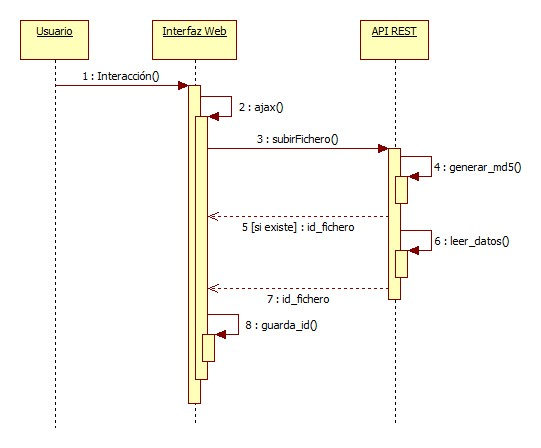
\includegraphics[scale=0.5]{figuras/sec_subir_fichero.jpg}
\caption{Diagrama de secuencia de la subida de ficheros.}
\label{fig:sec_subir_fichero}
\end{figure}

\item En la figura \ref{fig:sec_subir_fichero} podemos ver el diagrama de secuencia para la subida de ficheros de datos. Los objetos Interfaz Web y API REST representan a aquellos ficheros que componen la interfaz web (documentos HTML, CSS, JavaScript etc.) y aquellos que constituyen los servicios web REST (fichero de los servicios y la librería Bottle) respectivamente. Así mismo, la clase \textit{LimitedSizeDict} representa la clase utilizada para limitar el número de ficheros subidos (diccionario con límite de elementos). En primer lugar, el usuario interacciona con la interfaz, donde pulsa el botón para subir un fichero. En la ventana emergente, selecciona el fichero y pulsa el botón \textit{Subir fichero}. Esto desencadena una llamada AJAX al servicio de subida de ficheros del API REST: \textit{subir\_fichero()}. Esta llamada AJAX añade varios parámetros, como el contenido del fichero, el tipo de llamada a realizar (en este caso POST, pues se envían datos al servidor) o el tipo de datos que se esperan de vuelta (que para este proyecto siempre será JSON, como se indicó en el capítulo \ref{arquitecturayh}). Una vez en el servicio web, se obtiene el contenido del fichero especificado en la llamada AJAX con \textit{obtener\_fichero()}. Sobre este contenido, se aplica un algoritmo de reducción criptográfico denominado MD5: \textit{generar\_md5()}, que nos proporciona una clave única para el fichero que lo diferenciará de cualquier otro. Una vez obtenida esta clave, se consulta si existe dicho fichero: \textit{recuperar\_fichero(id)}. Si existe, se devuelve el identificador (en formato JSON) a la aplicación web, que se encargará de guardar en la sesión este identificador para su posterior uso: \textit{guardar\_id(id)}. Si no existe en el diccionario, entonces se invoca a la función \textit{leer\_datos(contenido)}, que determinará si el formato es adecuado y generará un JSON del contenido. Si el formato es adecuado este JSON es almacenado en el diccionario de ficheros con \textit{almacenar(datos)} y finalmente se devolverá el identificador a la interfaz web.


\begin{figure}[H]
\centering
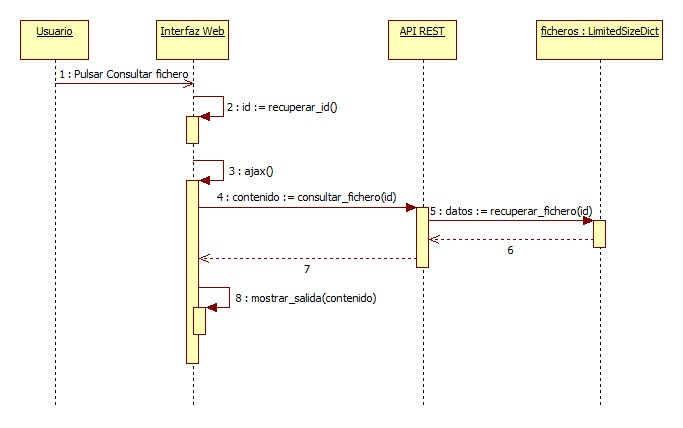
\includegraphics[scale=0.5]{figuras/sec_consultar_fichero.jpg}
\caption{Diagrama de secuencia de la consulta de ficheros.}
\label{fig:sec_consultar_fichero}
\end{figure}

\item En la figura \ref{fig:sec_consultar_fichero} se muestra el diagrama de secuencia para la consulta del fichero. Aquí, en primer lugar el usuario pulsa el botón de \textit{Consultar fichero}. Luego, la interfaz web recupera el identificador de fichero actual almacenado en la sesión: \textit{recuperar\_id()}. A continuación, se realiza la llamada AJAX al servicio web de consulta de ficheros. Esta llamada se diferencia de la anterior en que el método empleado es GET y no POST, pues únicamente se requiere un JSON (contenido del fichero). La llamada al servicio lleva como parámetro obligatorio el identificador del fichero: \textit{consultar\_fichero(id)}. El servicio recupera los datos del fichero: \textit{recuperar\_fichero(id)}, y devuelve el contenido a la interfaz, que se encarga de representar los datos en una tabla y mostrarlos mediante \textit{mostrar\_salida(contenido)}.

\begin{figure}[H]
\centering
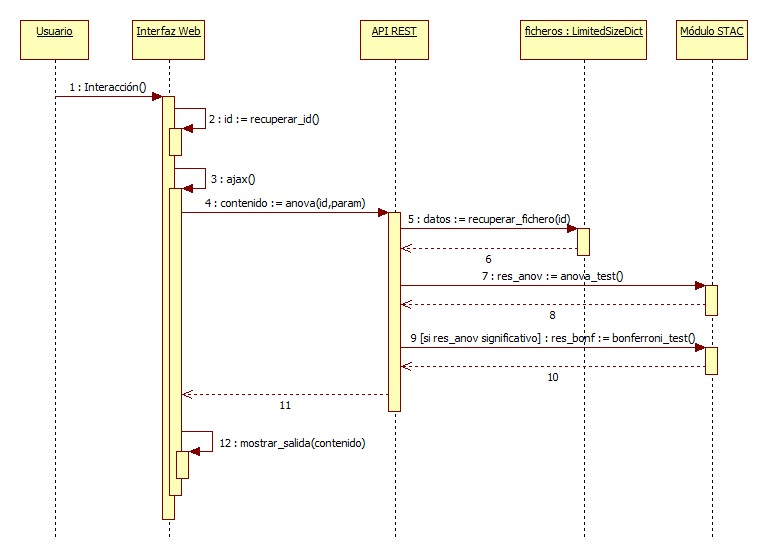
\includegraphics[scale=0.5]{figuras/sec_anova.jpg}
\caption{Diagrama de secuencia del test de ANOVA.}
\label{fig:sec_anova}
\end{figure}

\item La realización del test paramétrico ANOVA se muestra en el diagrama \ref{fig:sec_anova}. En este caso, el usuario accede a la sección de ANOVA en el apartado de test paramétricos, selecciona las opciones disponibles y aplica el test. La llamada al servicio, además del identificador del fichero, en este caso podría llevar más parámetros, como se muestra en la llamada a la función del servicio: \textit{anova(id,param)}. Estos parámetros se muestran en la sección \ref{dis_api}. En este caso, se tiene como parámetro opcional únicamente el nivel de significancia ``alpha". Una vez dentro del servicio web para ANOVA se accede al contenido del fichero de datos almacenado en el diccionario: \textit{recuperar\_fichero(id)} y se procede a realizar la llamada al test estadístico del módulo STAC: \textit{anova\_test()}. Los argumentos para los test se muestran en la sección \ref{dis_py}. Una vez obtenidos los datos (siempre en formato JSON), si el resultado de la prueba de ANOVA es estadísticamente significativa, se procede a aplicar el test POST-HOC de Bonferroni. Una vez aplicados los test se devuelve un JSON desde la API REST a la interfaz web con los resultados. Aquí nuevamente mediante \textit{mostrar\_salida(contenido)} se muestran los resultados del test de ANOVA en una tabla y, si hay resultados para el test POST-HOC de Bonferroni, se genera otra tabla para estos resultados.

\begin{figure}[H]
\centering
\begin{adjustwidth}{-5em}{-5em}
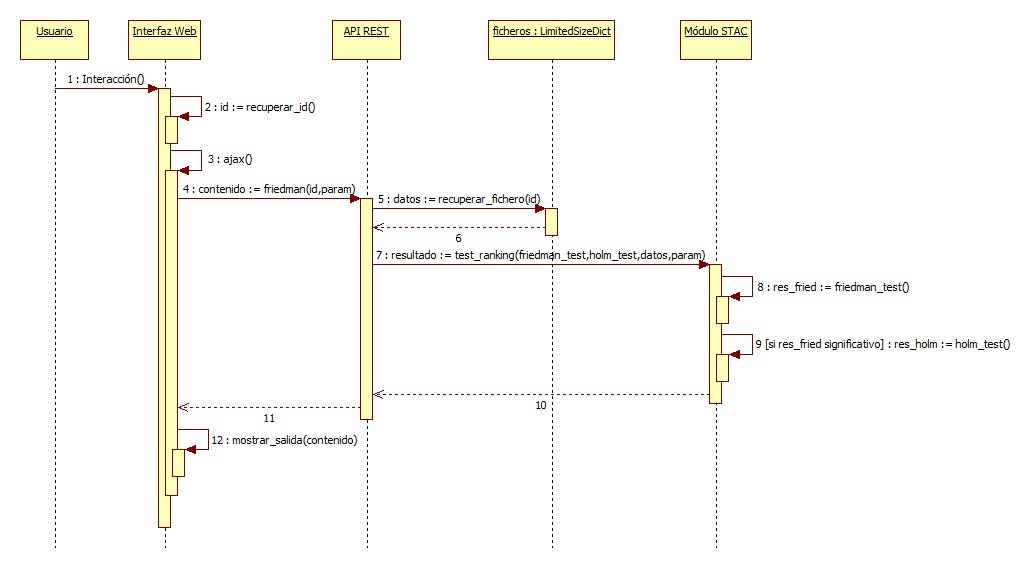
\includegraphics[scale=0.5]{figuras/sec_ranking.jpg}
\caption{Diagrama de secuencia de los test no paramétricos de ranking.}
\label{fig:sec_ranking}
\end{adjustwidth}
\end{figure}

\item En el diagrama de la figura \ref*{fig:sec_ranking} podemos ver el diagrama de secuencia para la realización de test de ranking. En este caso, la interacción del usuario con la interfaz implica posicionarse en la sección de test de ranking dentro de los test no paramétricos y seleccionar las opciones de aplicación de un test determinado. En este diagrama se muestra el ejemplo para la realización del test de Friedman junto con el test POST-HOC de Holm. Sin embargo, esto sería aplicable para todos los test de ranking. Como se ha dicho anteriormente, tanto los parámetros de los servicios como los parámetros de las funciones de los test se muestran en las secciones \ref{dis_api} y \ref{dis_py} respectivamente. Este tipo de test se caracterizan por la invocación de la función \textit{test\_ranking(friedman\_test,holm\_test,datos,param)}, que permite separar los test POST-HOC de los test de ranking, evitando tener que pasar como argumento al test POST-HOC el test de ranking realizado previamente. Dentro de esta función, se realiza el test de Friedman: \textit{friedman\_test()} y si su resultado es estadísticamente significativo, se realiza el test POST-HOC de Holm: \textit{holm\_test()}, de forma similar al test de ANOVA.

\item Por último, en la figura \ref{fig:sec_scipy} se muestra el caso de la aplicación de test pertenecientes a la librería SciPy. Por tato, se incluye el objeto Módulo SciPy. El diagrama muestra como caso de ejemplo la aplicación del test de normalidad de Shapiro-Wilk: \textit{shapiro()}. Este test se aplica para cada uno de los algoritmos de aprendizaje automático presentes en el fichero de entrada, con el objetivo de determinar si los datos obtenidos por cada algoritmo siguen una distribución normal. Además, se muestra una segunda interacción del usuario, en la cual éste en la pantalla de visualización de resultados de los test pulsa el botón de \textit{Exportar a formato \LaTeX}. Como se puede apreciar, la interfaz web en este caso invocaría  a la función \textit{exportTableToLaTeX()} para generar el contenido. Ocurriría lo mismo en caso de la exportación de resultados a formato CSV (con la función \textit{exportTableToCSV()}).

\begin{figure}[H]
\centering
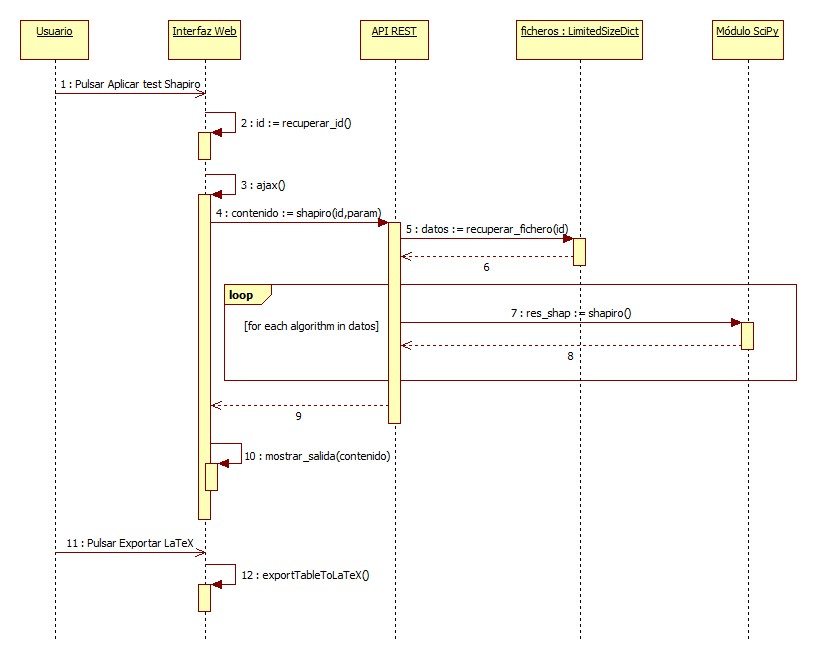
\includegraphics[scale=0.5]{figuras/sec_scipy.jpg}
\caption{Diagrama de secuencia de los test de SciPy.}
\label{fig:sec_scipy}
\end{figure}

\end{enumerate}
